%%%%%%%%%%%%%%%%%%%%%%%%%%%%%%%%%%%%%%%%%
% FRI Data Science_report LaTeX Template
% Version 1.0 (28/1/2020)
% 
% Jure Demšar (jure.demsar@fri.uni-lj.si)
%
% Based on MicromouseSymp article template by:
% Mathias Legrand (legrand.mathias@gmail.com) 
% With extensive modifications by:
% Antonio Valente (antonio.luis.valente@gmail.com)
%
% License:
% CC BY-NC-SA 3.0 (http://creativecommons.org/licenses/by-nc-sa/3.0/)
%
%%%%%%%%%%%%%%%%%%%%%%%%%%%%%%%%%%%%%%%%%


%----------------------------------------------------------------------------------------
%	PACKAGES AND OTHER DOCUMENT CONFIGURATIONS
%----------------------------------------------------------------------------------------
\documentclass[fleqn,moreauthors,10pt]{ds_report}
\usepackage[english]{babel}

\usepackage{comment}

\graphicspath{{fig/}}




%----------------------------------------------------------------------------------------
%	ARTICLE INFORMATION
%----------------------------------------------------------------------------------------

% Header
\JournalInfo{FRI Data Science Project Competition 2023}

% Interim or final report
%\Archive{Interim report} 
\Archive{Final report} 

% Article title
\PaperTitle{Feature selection on large and sparse datasets} 

% Authors (student competitors) and their info
\Authors{Leon Hvastja, Amadej Pavšič}

% Advisors
\affiliation{\textit{Advisors: Jure Demšar, Blaž Mramor, Blaž Škrlj}}

% Keywords
\Keywords{feature selection, feature ranking, machine learning, big data, sparse features}
\newcommand{\keywordname}{Keywords}


%----------------------------------------------------------------------------------------
%	ABSTRACT
%----------------------------------------------------------------------------------------

\Abstract{
This project centers on feature selection in large datasets, specifically within Outbrain's web recommendations platform. We engaged various selection methods and developed an evaluation pipeline for efficient testing across multiple models, sampling regimes and other parameters. Our performance assessments were founded on a tailored metric we developed from the Jaccard index.
% Two ground truth rankings, one derived from a simultaneous ranking of all features and the other from a forward feature selection process, were provided by the company. Our objective was to align our methods with these reference rankings. 
Two separate ground truth rankings were provided by the company and our objective was to align our methods with these.
Random forests emerged as the superior approach, balancing accuracy and computation time. We developed a novel technique, using the Borda count voting system on rankings from random data subsamples to determine feature importance. This method enabled us to use extremely small samples of the data to achieve greater accuracy than rankings derived from the entire dataset.
%
The smallest subsampling rates observed the greatest gain in their performance.
% Using this technique, we observed an increase in accuracy with larger subsamples, the smallest subsamples recording the most significant gain. 
This approach also led to a time-efficient solution with markedly lower variance in ranking accuracy, strengthening our evaluation confidence. 
%
%Our method provides a time-efficient solution that is not only more accurate but also exhibits lower variance. 
These findings suggest a new method that utilizes small data samples to yield high-quality evaluations with lower variance in feature selection, enabling Outbrain to conduct more reliable feature evaluations swiftly, while using less data, thereby enhancing their existing methods.
}

%----------------------------------------------------------------------------------------

\begin{document}

% Makes all text pages the same height
\flushbottom 

% Print the title and abstract box
\maketitle
% Removes page numbering from the first page
\thispagestyle{empty}

%----------------------------------------------------------------------------------------
%	ARTICLE CONTENTS
%----------------------------------------------------------------------------------------


\begin{figure*}[!ht]
	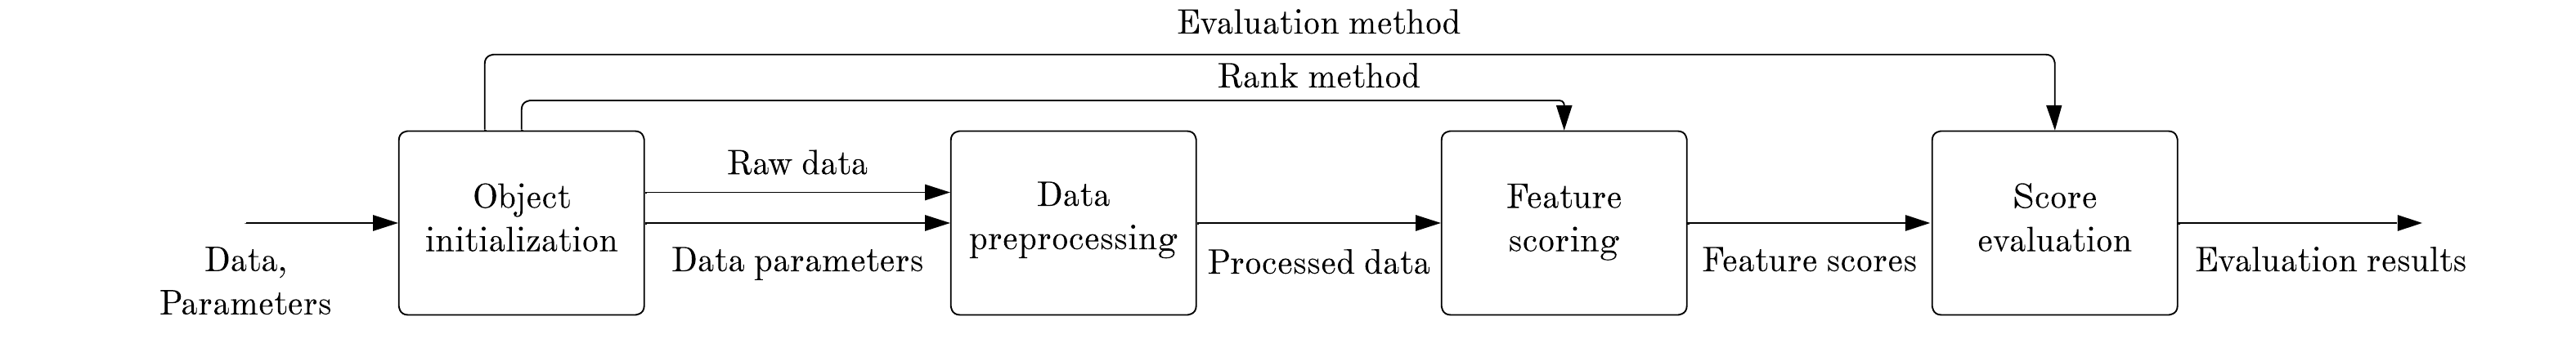
\includegraphics[width=\linewidth]{img/block_diagram_cropped.png}
    \captionsetup{justification=centering}
	\caption{\textbf{A visualization of our feature ranking and evaluation pipeline.} It enables streamlined evaluation of various ranking algorithms with customizable parameters and subsampling regimes.}
	\label{fig:block_diagram}
\end{figure*}


\section*{Introduction}

Feature selection is the process of reducing the number of input variables when building a predictive model. The aim is to reduce computational costs and, in some cases, also improve model accuracy.

Our project aimed to explore feature selection methods for Outbrain, a web recommendation platform. 
%
In this domain, it's common to encounter vast quantities of data characterized by sparse or completely useless features, meaning that a lot of the information may be missing, irrelevant or uninformative. This presents a challenge in terms of efficiency and cost-effectiveness, as running predictive models on such extensive, largely unrefined data can be both time-consuming and costly. Consequently, feature selection emerges as an indispensable component of the company's workflow.
%

%They provided us with data from their regular operations, which was typically large, sparse, and required time-efficient use. The dataset underwent minimal preprocessing specific to our project. We were also provided with their internally generated feature scores to use as a reference.

They provided us with a dataset from their regular operations, which they minimally preprocessed for our use. We were also provided with their internally generated feature scores to use as the ground truth.


We hypothesized that simpler models could produce quick feature selection results, but models that accounted for feature interactions would be more accurate at the expense of longer computations.

The main goal of our project was thus the development of an efficient and intelligent feature selection approach given the specifics and constraints of Outbrain's domain of work.

	% These latex files are intended to serve as a the template for the FRI Data Science Project Competition. If you find mistakes in the template or have problems using it, please consult Jure Demšar (\href{mailto:jure.demsar@fri.uni-lj.si}{jure.demsar@fri.uni-lj.si}).
	
	% In the Introduction section you should write about the relevance of your work (what is the purpose of the project, what will we solve) and about related work (what solutions for the problem already exist). Where appropriate, reference scientific work conducted by other researchers. For example, the work done by Demšar et al. \cite{Demsar2016BalancedMixture} is very important for our project. The abbreviation et al. is for et alia, which in latin means and others, we use this abbreviation when there are more than two authors of the work we are citing. If there are two authors (or if there is a single author) we just write down their surnames. For example, the work done by Demšar and Lebar Bajec \cite{Demsar2017LinguisticEvolution} is also important for successful completion of our project.


%------------------------------------------------


\section*{Methodology}

\subsection*{Rank and Evaluation Pipeline}

We developed a feature ranking and evaluation framework that streamlines our algorithm testing process. The framework's primary function is to generate a ranking, which is an ordered list of features based on their importance, and an evaluation of that ranking. This pipeline handles data reading, pre-processing, feature score calculations, and evaluations against our ground truth. To provide a visual representation of the pipeline, we have included a flowchart in Figure \ref{fig:block_diagram}.

% However, due to the large size of our dataset, one of the main challenges is managing computational complexity. Some ranking algorithms take hours to process even a small portion of the dataset, making it infeasible to apply them to the entire dataset. To tackle this issue, we plan to use our framework to run batches of evaluations on a high-power computing network. While this will allow us to perform more computations, it will not completely solve our computing complexity problem.

During our preprocessing stage, we employ data factorization to convert the original dataset's values, generated by a hashing function, into categorical representations. These categories are then re-encoded as integers from 0 to n, where n represents the count of unique feature values.

To optimize computational load, we incorporated random subsampling by rows into our framework. In order to ensure reproducibility, a seed value is passed to the sampling process and logged in the output. The aim was to use this approach to gain insight into the behavior of our feature scoring algorithms on datasets of varying sizes, and possibly identify an effective subsampling strategy for very large datasets.

\subsection*{Ranking algorithms}

The algorithms we chose to base our approaches on fall into the following two categories: a) \textbf{filter methods} (rank features independently of any machine learning algorithm) and b) \textbf{wrapper methods} (use ML algorithms to implicitly rank features). A complete list of used algorithms is shown in Figure \ref{fig:all_algos}.

Our selection of filter methods included widely-used approaches that rely on statistical tests, along with a suite of feature ranking algorithms derived from the Relief algorithm. The latter is capable of identifying feature interactions, but its time complexity is significantly higher than that of other methods.

The wrapper methods used some of the most common and fast ML models such as random forests and XGBoost. The aim here was to build simple models and extract the implicit feature importance from the model.


\subsection*{Ranking Evaluation}

We had two distinct methods for establishing ground truth rankings: a) \textbf{single feature model-based ranking}, where individual models are built for each feature separately, and b) \textbf{forward selection ranking}, which iteratively adds the highest-performing features one at a time to progressively build a model that uses all features.

To evaluate our rankings, we used the \textbf{Jaccard index}. We generate a score by comparing subsets of sequential elements derived from our ranking with the corresponding subsets from the ground truth ranking. More specifically, the score at index $k$ in our evaluation corresponds to the Jaccard index computed for the subsets extending from index 1 up to index $k$. For a visual representation of this evaluation and its corresponding curve, refer to \figurename~\ref{fig:evaluation_comparison}.
 

\subsection*{Baseline}

Due to the way we evaluated our rankings it's not possible to score 0 over all indices. To correct for this we used a baseline which is a set of expected values of a random permutation across all values of $k$. We defined the baseline values using the following equation:
\begin{equation}
    E[k] = \sum_{i=1}^{k} \frac{\binom{k}{i} \cdot \binom{T-k}{k-i} \cdot \left(\frac{i}{2k-i}\right)}{\binom{T}{k}} \label{eq:baseline},
\end{equation}
where $E[k]$ denotes the expected value of the Jaccard score for a random permutation at index $k$, and $T$ stands for the total number of features.

We introduced the \textbf{Baseline Corrected Score (BCS)}, specifically tailored to our use case in order to provide a concise representation of algorithm performance. Initially, we condense the array of Jaccard index scores obtained from our evaluation pipeline into a single value representing the area under the \textbf{evaluation curve}. Subsequently, we apply a linear transformation to ensure that the baseline performance corresponds to zero, while a perfect ranking receives a score of 1. A perfect ranking is possible only if there is no noise in the data or our algorithm makes an extremely lucky guess. Note that a negative score is possible if an algorithm performs worse than an algorithm picking random features.



\begin{figure*}[!ht]
	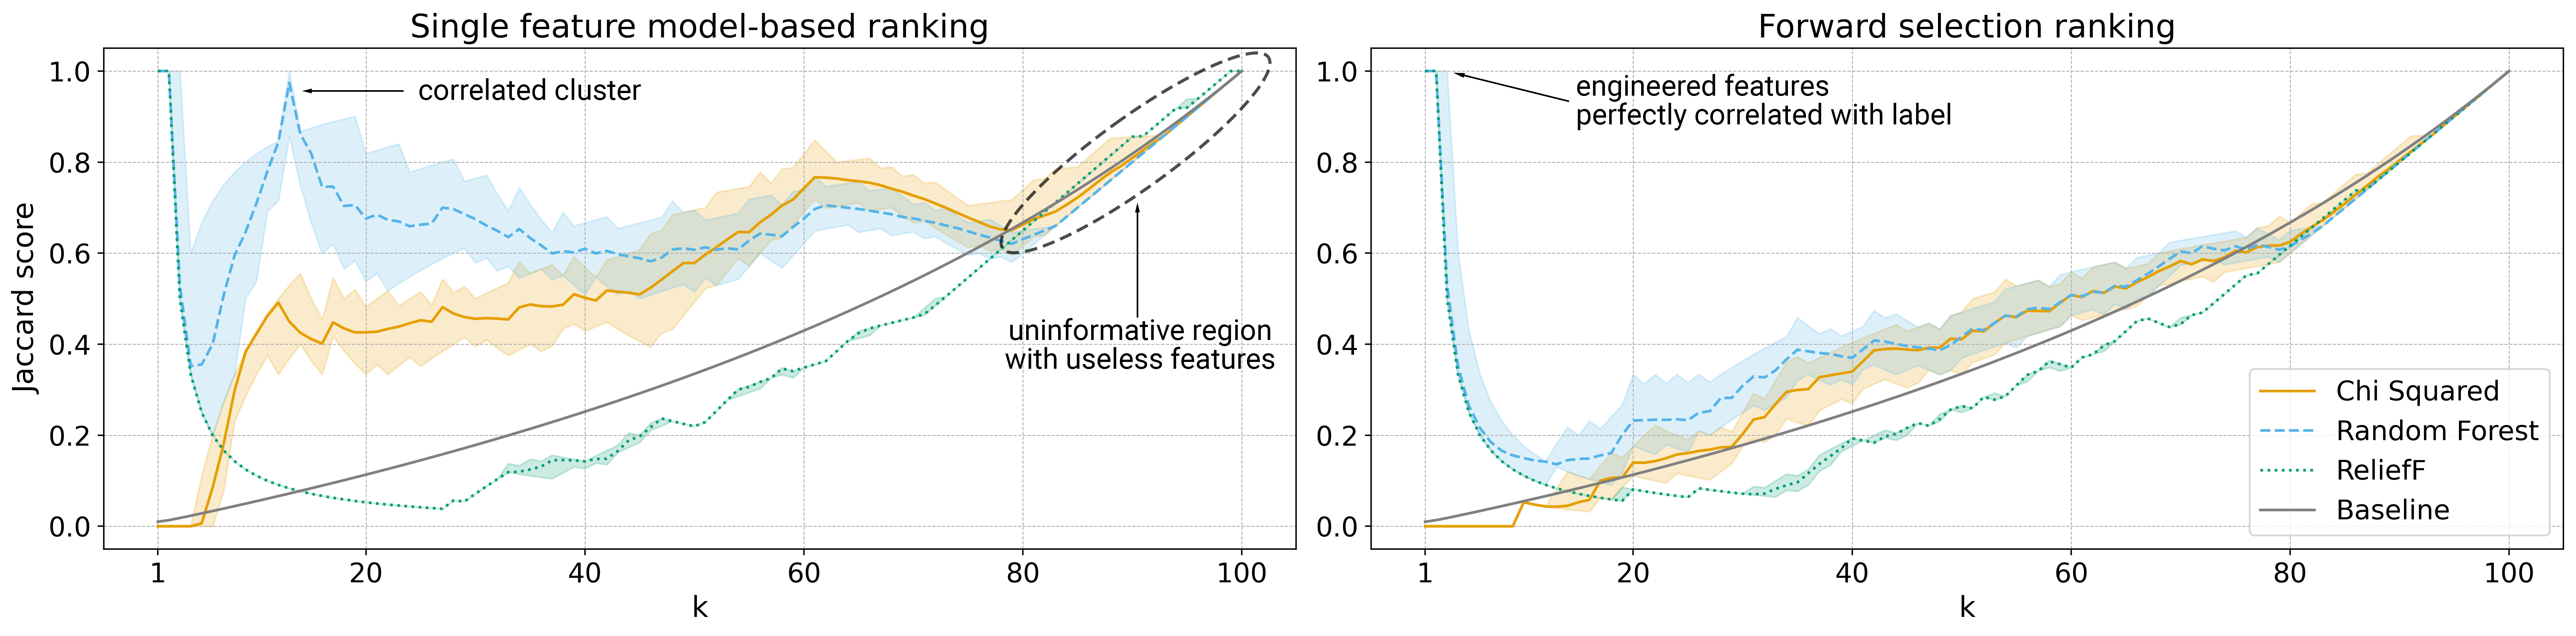
\includegraphics[width=\linewidth]{img/ranking_comparison_chosen_annotated.png}
	\caption{\textbf{Ranking evaluation comparison for 100 runs.} Jaccard score for each top k features for three different ranking algorithms with visualized uncertainty and and our analytically determined baseline.}
	\label{fig:evaluation_comparison}
\end{figure*}

\section*{Results}

\subsection*{Exploratory Data Analysis}

The main purpose of exploratory data analysis (EDA) was to familiarize ourselves with the data and start developing ideas for intelligent preprocessing. The dataset logs ad clicks and contains over 1.5 million data points with 100 features and a binary \textbf{label} indicating whether the ad was clicked or not. All features were anonymized with numerical labels such as \textbf{feature0}. The data contains only categorical features whose values come from feature hashing, making them impossible to interpret. There were no explicitly missing values in the dataset since these were also hashed into integers.

\textbf{Cardinality} was one of the crucial feature properties we analyzed in our EDA. We observed that 7 features contained only one unique value, rendering them uninformative. 8 features, as well as the label, were binary, while 20 features had more than 1000 unique values.

The label exhibited an 80-20 ratio, indicating a bias toward the ad not being clicked. Additionally, the features had varying value distributions, and we observed that 13 features had one highly prevalent value, occurring in over 90\% of the samples. We inferred that these values very likely represented missing values, implying that the corresponding features were quite sparse.




We used Pearson's correlation coefficient (PC) to examine the connections between features. Our observations unveiled sets of highly correlated attributes, some of which exhibited a negative association with the label.

It's worth noting that features 98 and 99 had a perfect correlation (PC = 1) with each other as well as with the label, effectively making them flawless predictors. These features were engineered into the data and were useful for the initial validation of our approaches as they are expected to be at the top of the feature rankings.


\subsection*{Visualizing ranking performance}

In \figurename~\ref{fig:evaluation_comparison} we visualize evaluation curves for three different ranking algorithms. The shaded areas represent the variability of runs with different subsampling seeds. We limited this visualization to three rankings with varying behavior for readability but they display characteristics that were recurring among all our algorithms.

First, let us consider the single feature model-based ranking evaluation (left). The most prominent pattern is the initial ledge with a steep drop-off. This is caused by the two engineered features that correlate perfectly with the label and is perhaps the most basic indicator of algorithm coherence. We included the chi-squared metric to show that in fact not all ranking algorithms put these features in first and second place as we would like.

Another pattern we observe is at the tail of our curve. All algorithms converge very close to the baseline at higher $k$ values. This occurs when the algorithms encounter non-informative features. Numerically they are indistinguishable so the ordering has no structure, they are ranked randomly so our evaluation curve converges to the baseline, which is equivalent to guessing. We call this the \textbf{uninformative region}. This property of our data guarantees no approach will be able to consistently achieve a perfect score.

The last major pattern that had a high rate of recurrence among different ranking algorithms was the local peak in the values of $k$ from 10 to 20. The cause is one of the correlated clusters of features that correlate negatively with the label that we found while performing EDA, many algorithms were able to correctly rank these features as important.

Unfortunately, no significant patterns occurred on the forward feature selection evaluation (right) for any of our tested algorithms. The only exception being detection of the two engineered features as before. The reason our rankings performed better than baseline is because of the intrinsic overlap between the two base truth rankings. At this point our conclusion was that none of our approaches were able to match the feature ranking from the forward selection method used by Outbrain. We instead shifted our focus to optimizing performance for single feature model-based ranking.

\begin{figure}[!h]
	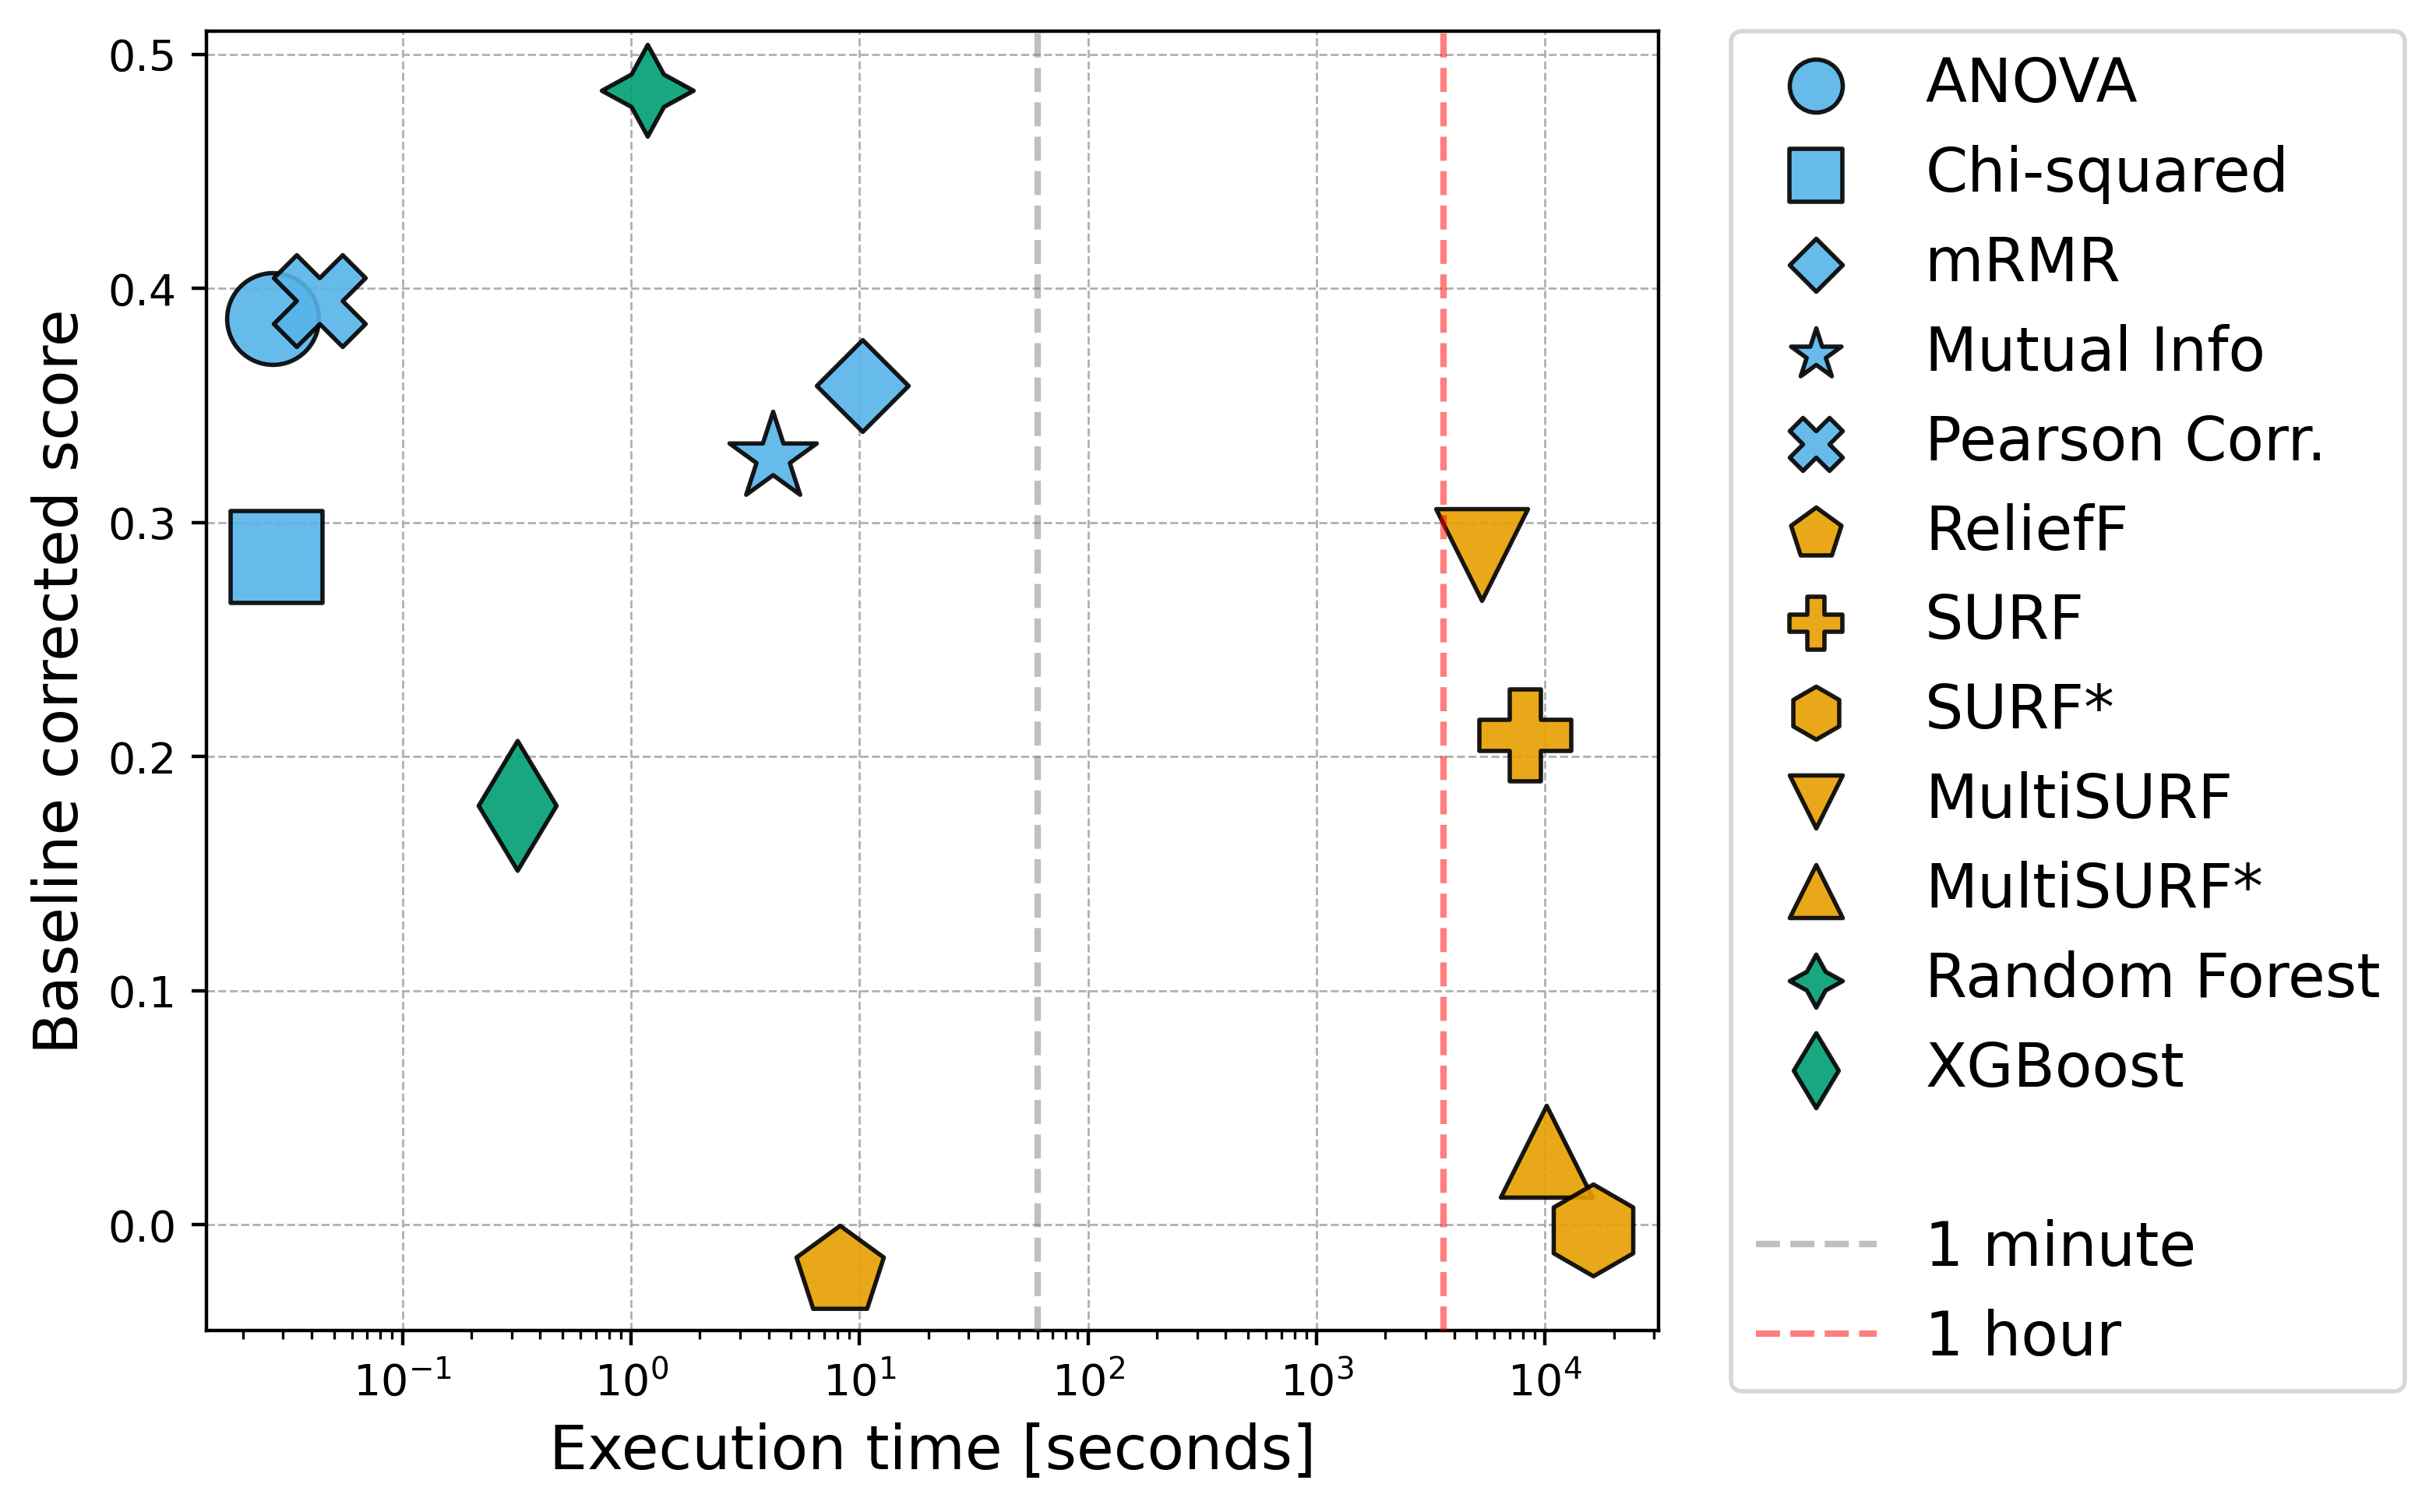
\includegraphics[width=\linewidth]{img/all_algos.png}
	\caption{\textbf{All algorithms' score and runtime comparison.} Results were obtained with 1\% subsampling.}
	\label{fig:all_algos}
\end{figure}

Next, we considered the algorithms' computational times versus their performance. The results are shown in \figurename~\ref{fig:all_algos}. The x-axis depicts time on a logarithmic scale, a reference point for one minute and one hour are shown for intuition. The algorithm with the highest baseline corrected score was the random forest model from the scikit-learn library. Despite some algorithms exhibiting slightly faster performance, the random forest model still met our feasibility threshold while maintaining higher levels of performance. Consequently, it was selected as the sole candidate for further exploration in our analysis.

% \begin{figure}[!h]
% 	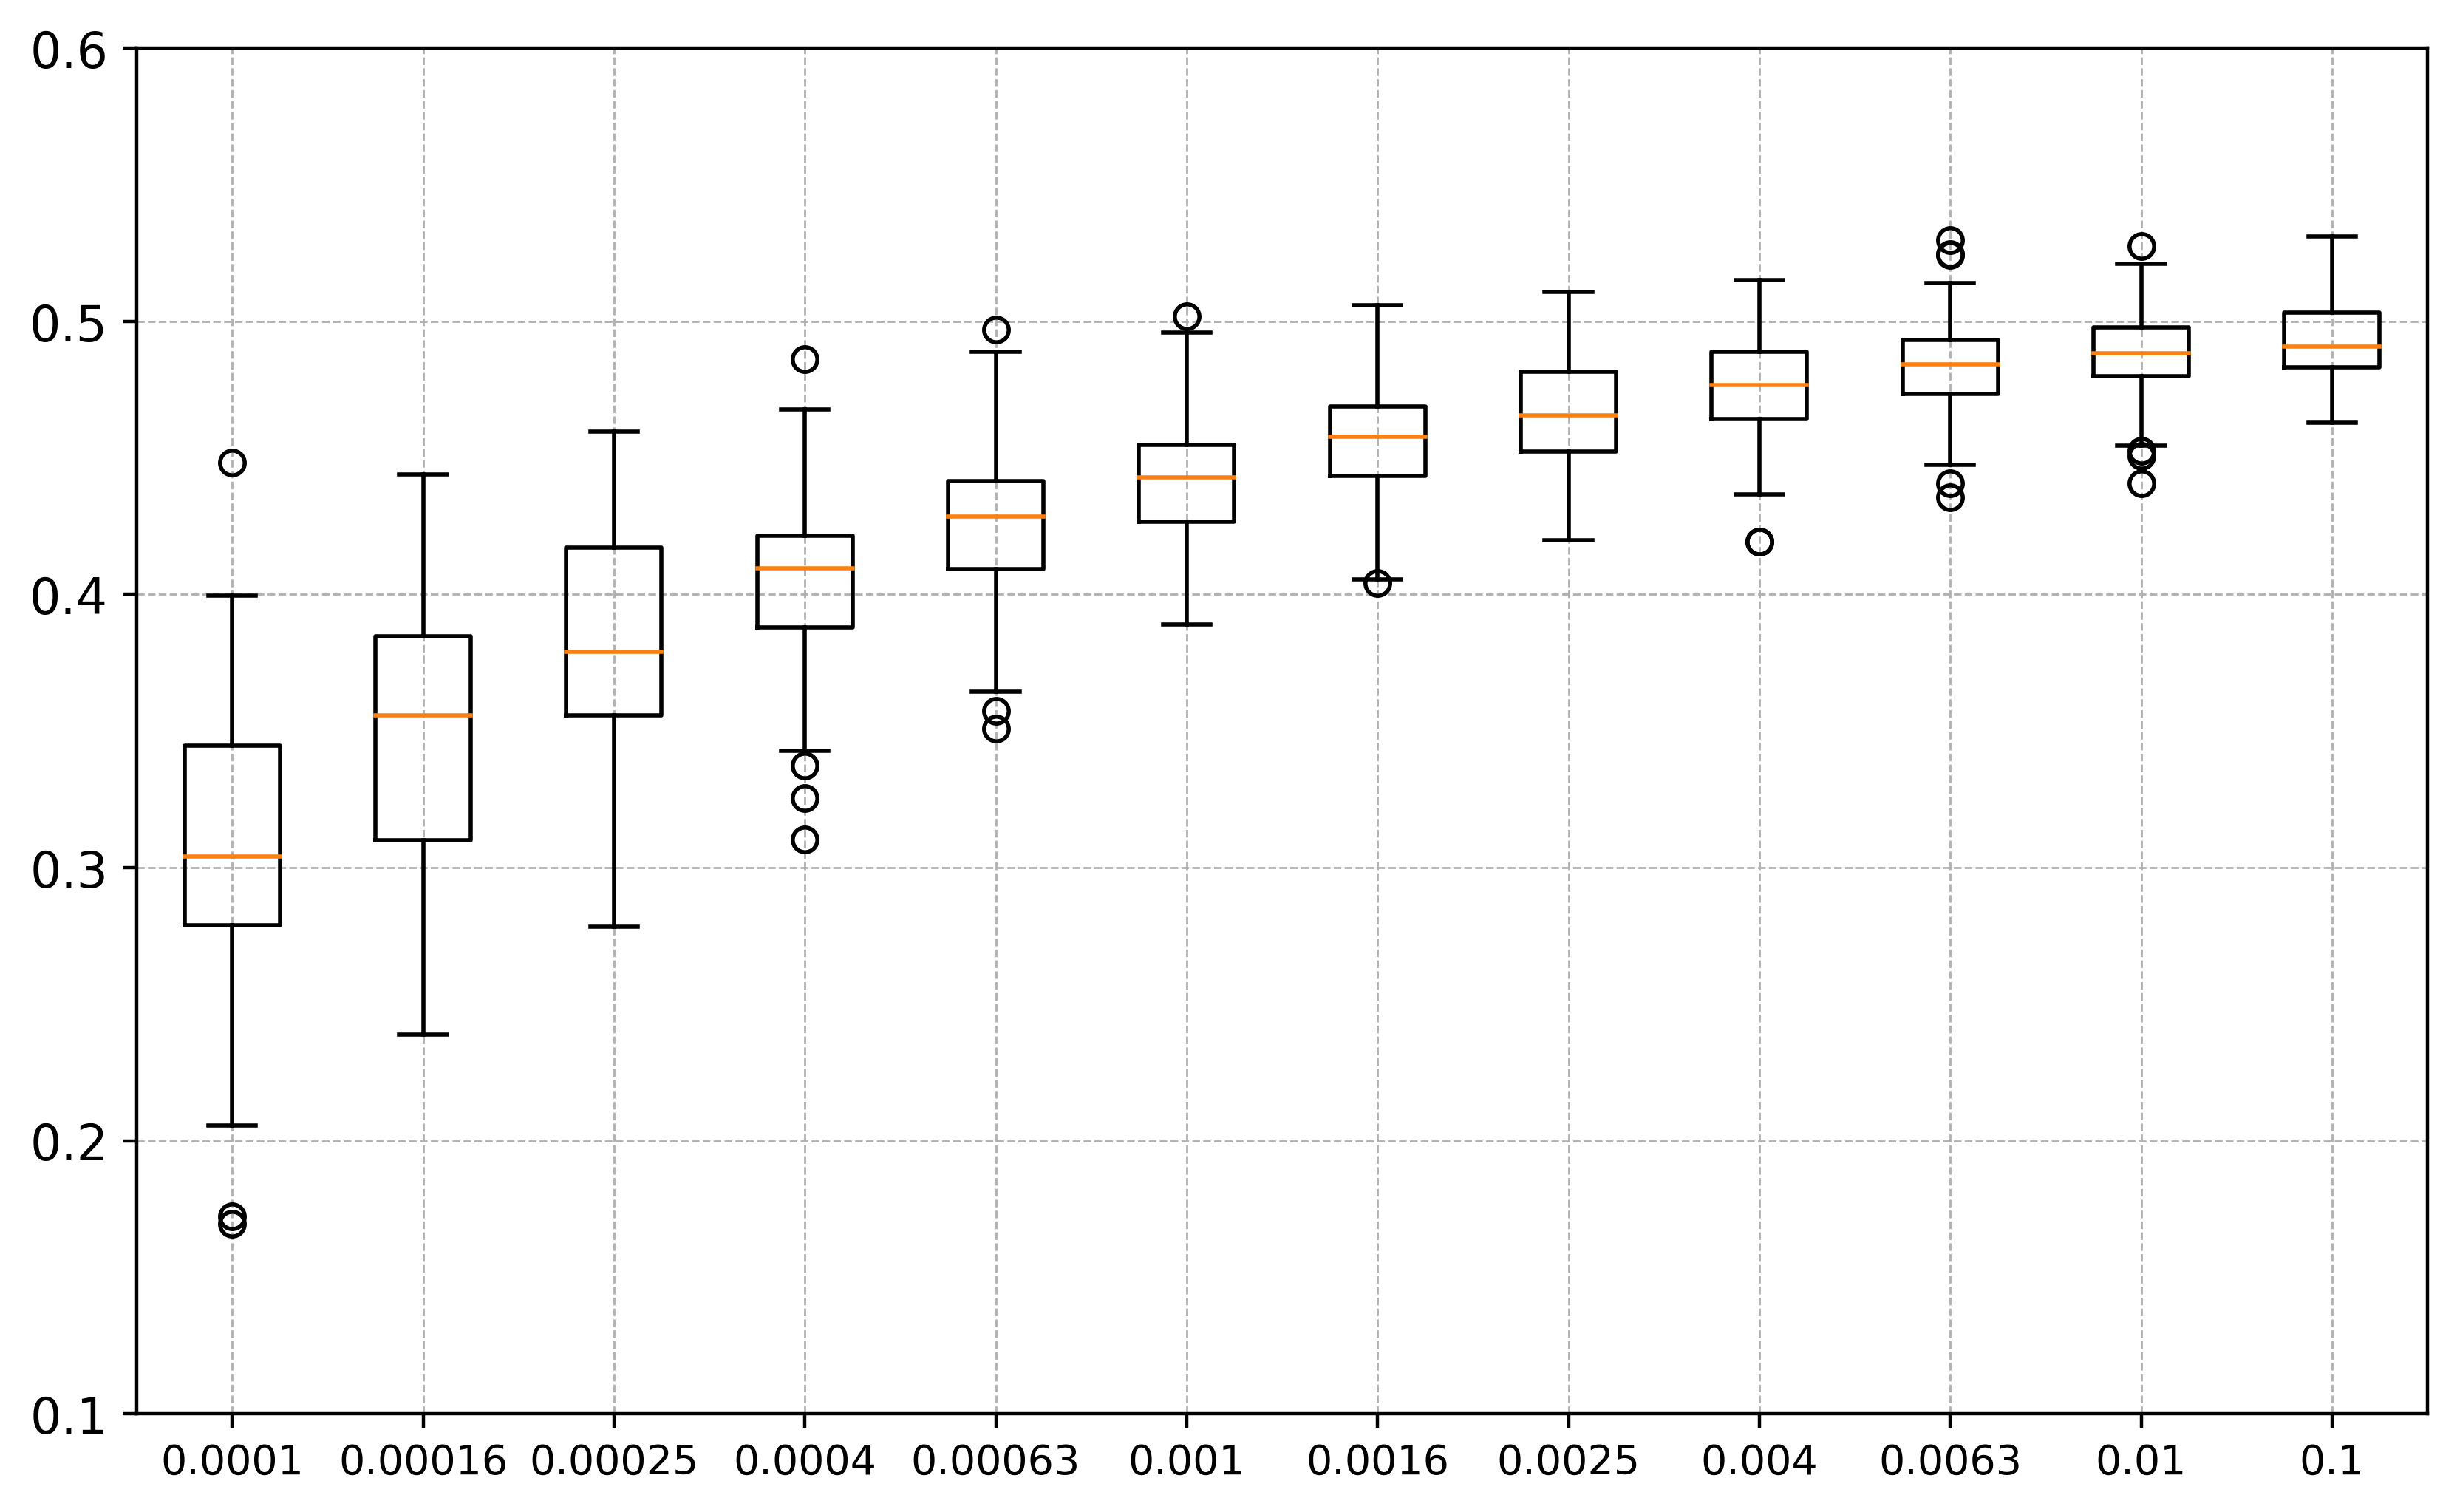
\includegraphics[width=\linewidth]{img/subsampling_boxplot.png}
% 	\caption{\textbf{Subsampling performance with different subsampling proportions.} .}
% 	\label{fig:subsampling_performance}
% \end{figure}

\subsection*{Optimal subsampling proportion}

To find the optimal sampling regime, we performed a number of evaluations with a wide range of different logarithmically spaced subsampling rates getting 100 different samples for each. The generated data's distributions are shown in \figurename~\ref{fig:RF_ensemble_vs_individual}, shown as \textbf{individual rankings}. We used bootstrapping to evaluate the uncertainty of the ensemble method. We can observe the mean BCS for the ensemble method outperforming significantly higher sample sizes of individual rankings while also having notably lower uncertainty.


\begin{figure}[!h]
	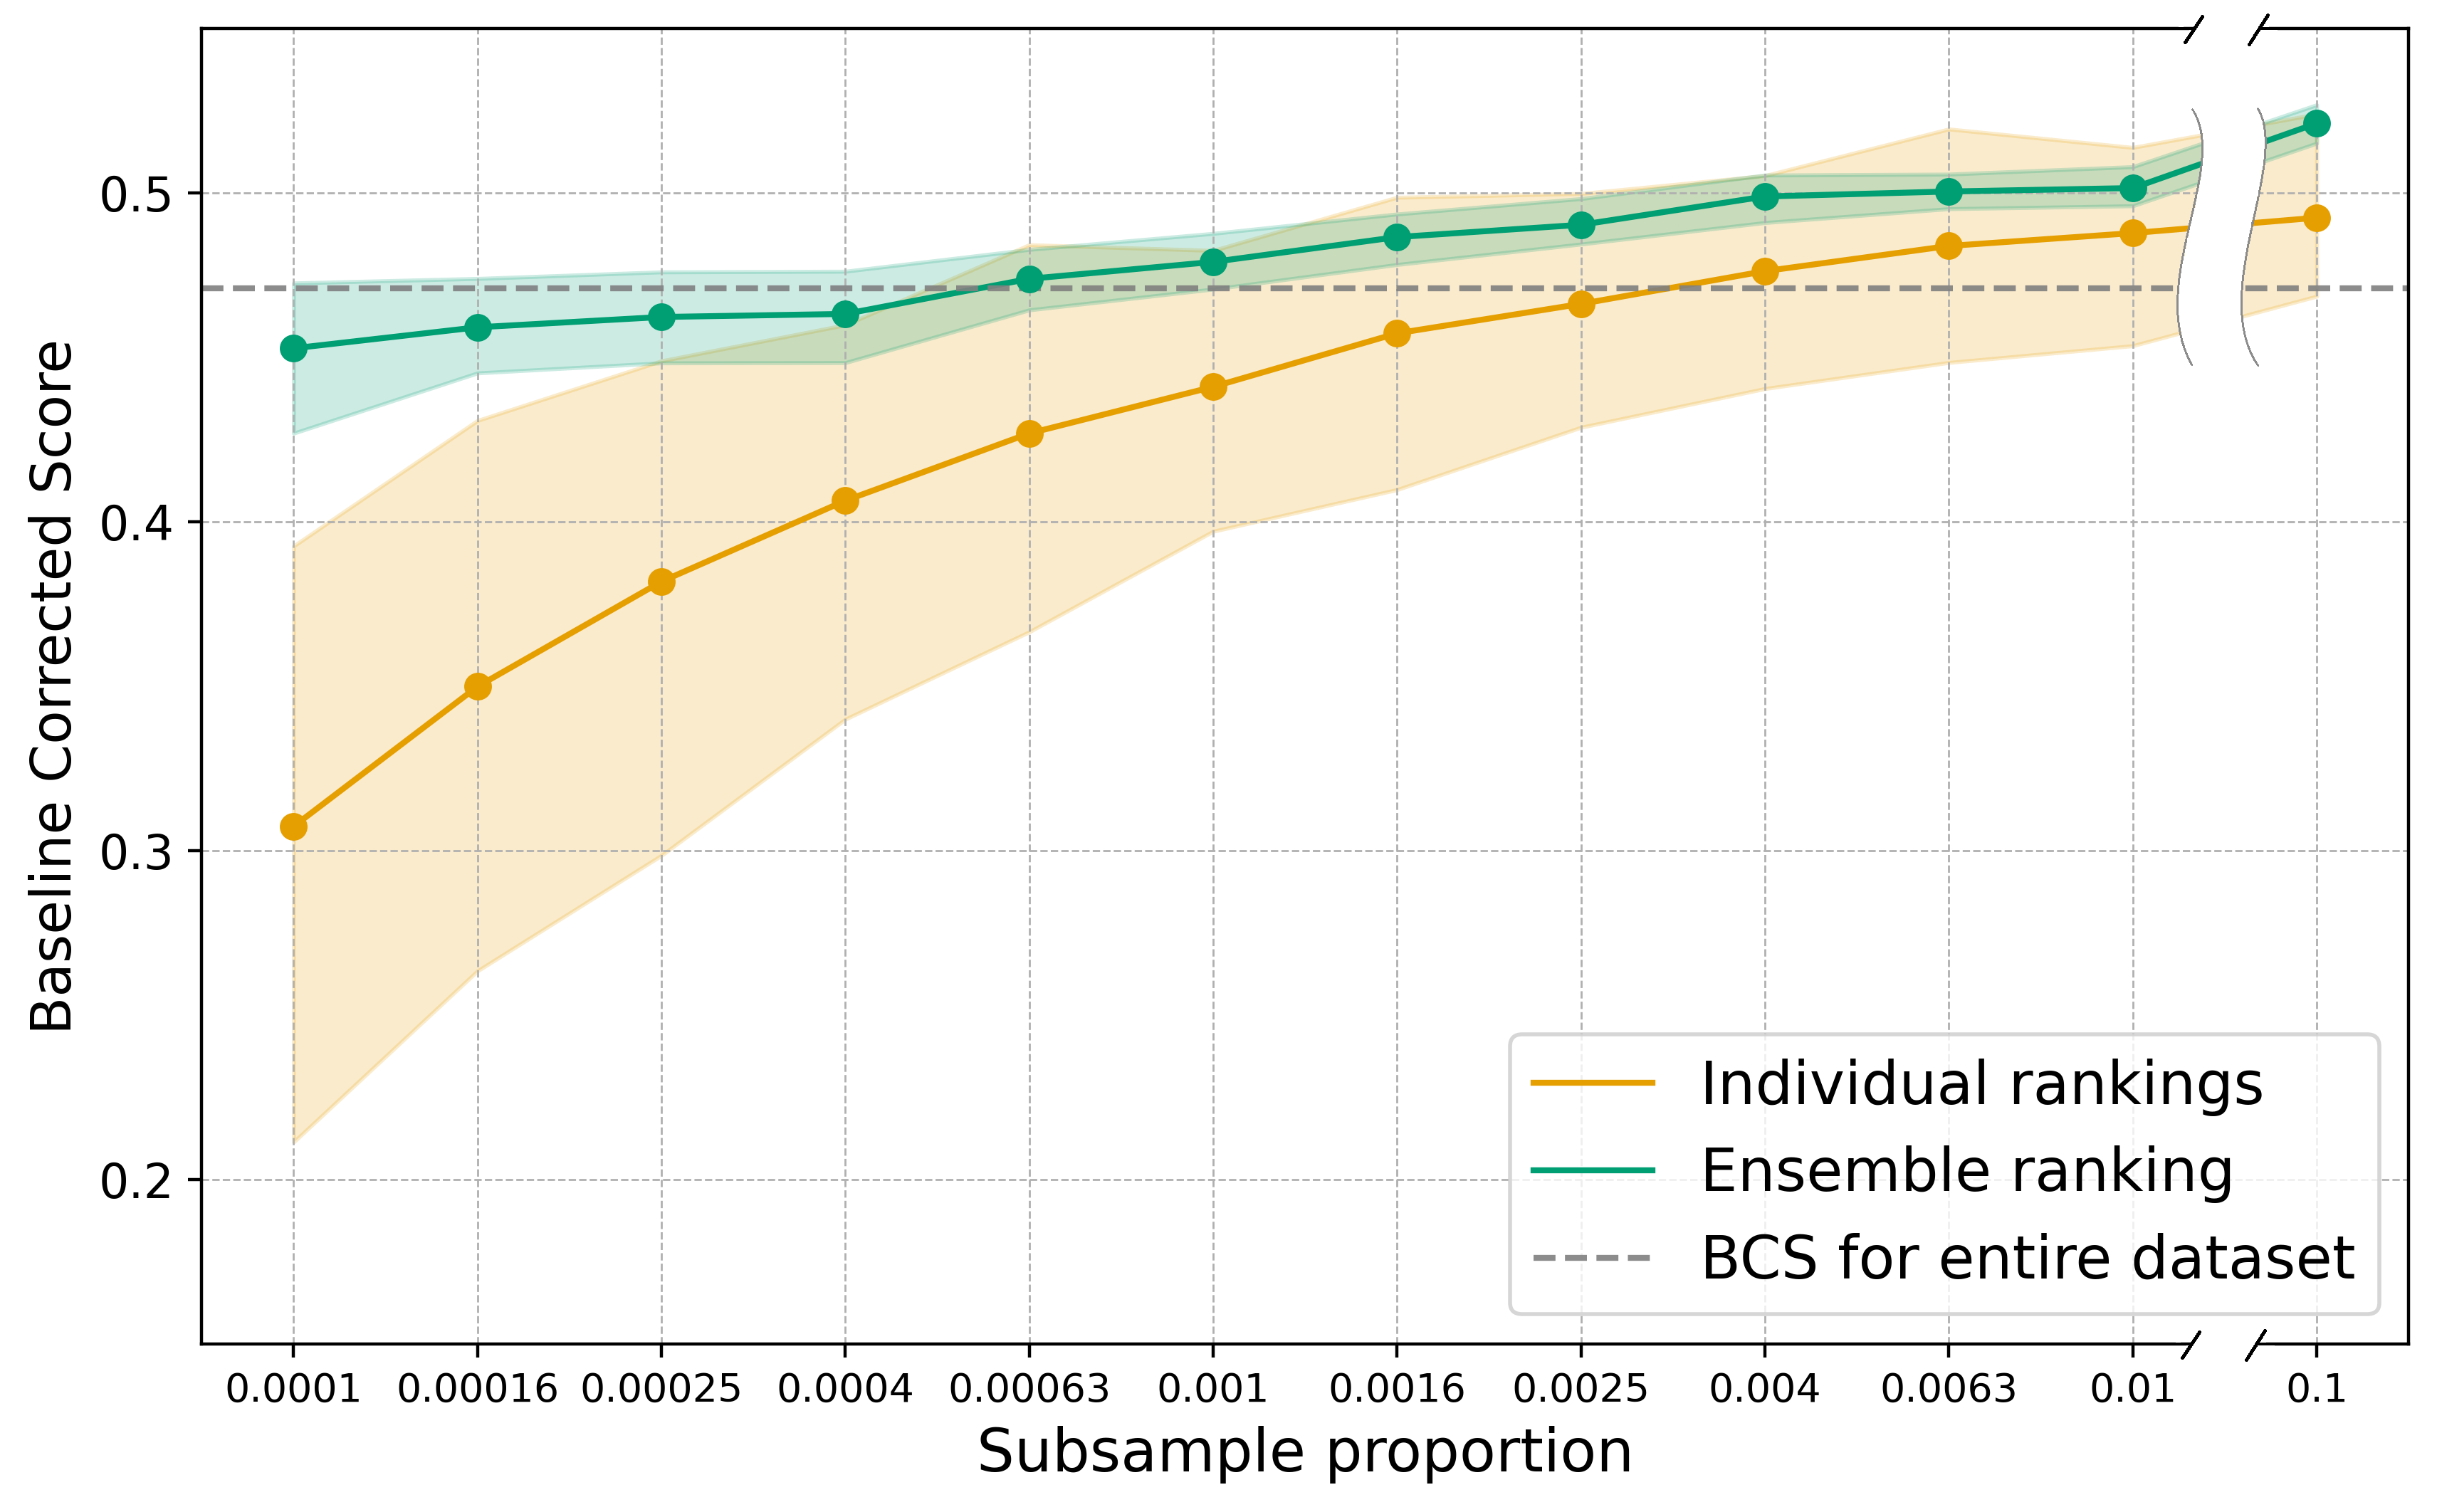
\includegraphics[width=\linewidth]{img/RF_bootstrap_results_ensemble_lines_broken_axis.png}
	\caption{\textbf{Comparison of individual and ensemble rankings scores over 100 runs with different subsamples.} Some results between 1 and 10\% subsampling are omitted.}
	\label{fig:RF_ensemble_vs_individual}
\end{figure}


\begin{figure}[!h]
	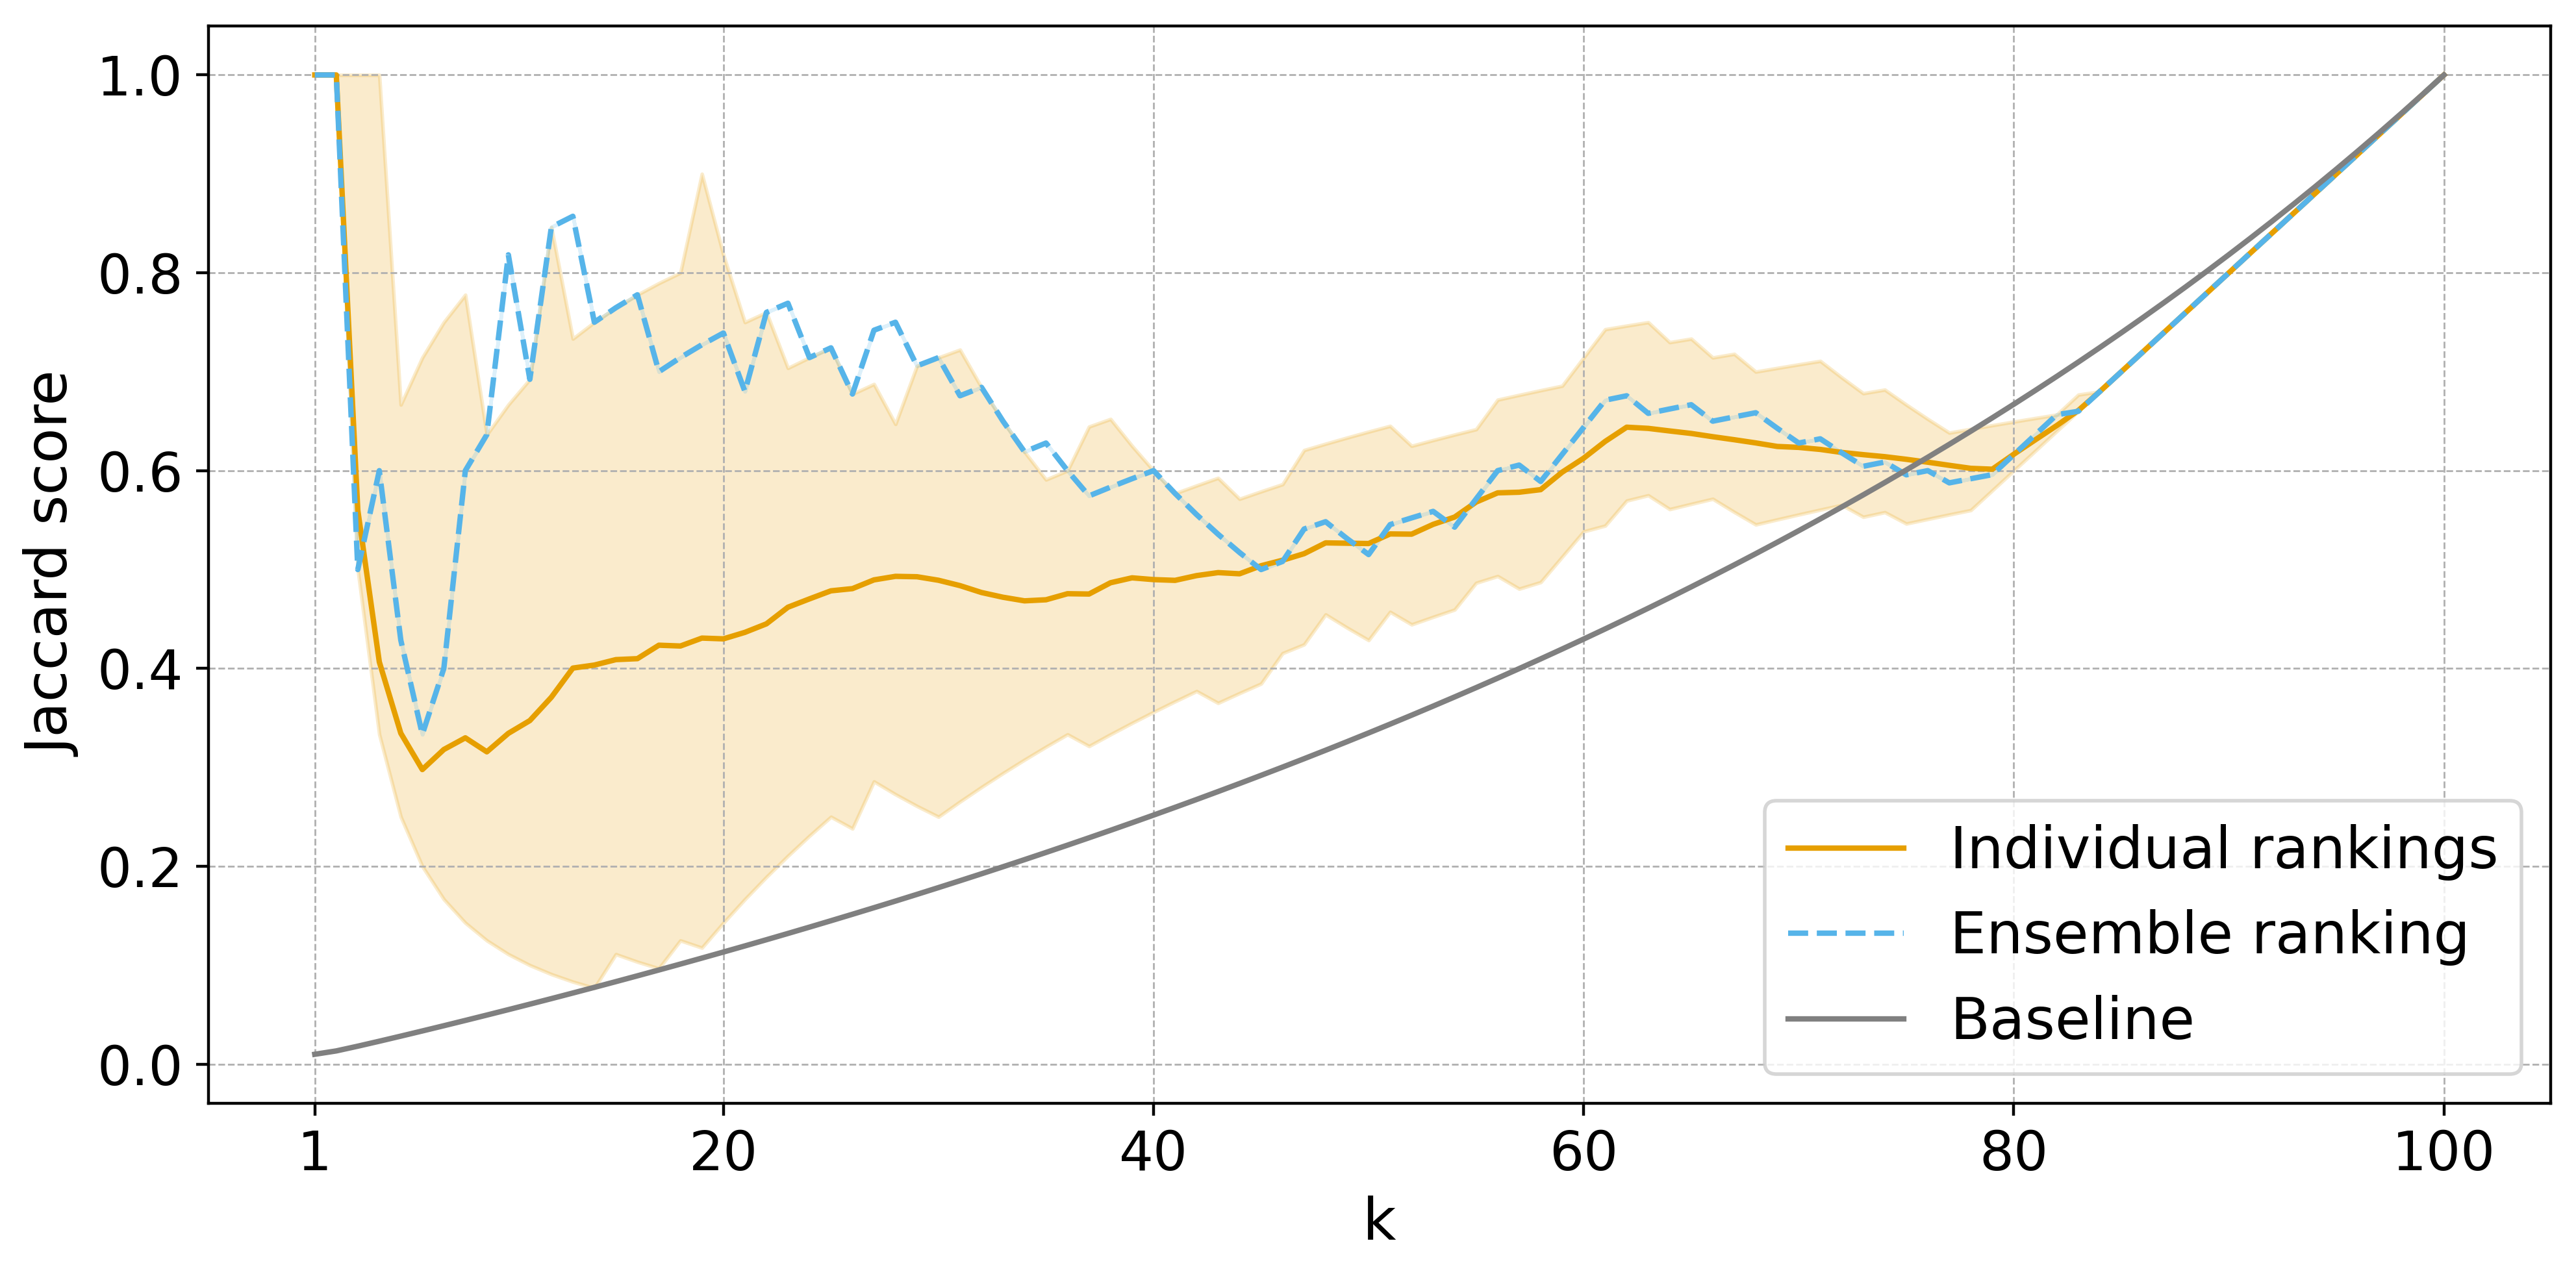
\includegraphics[width=\linewidth]{img/rf_performance_ensemble_vs_individual.png}
	\caption{\textbf{Random forest ranking scores over 100 runs with 0.01\% subsampling.} Comparison between individual and ensemble rankings using the same data.}
	\label{fig:rf_performance_ensemble_vs_individual}
\end{figure}

\subsection*{Ensemble technique}

Utilizing a version of the ensemble technique, we managed to achieve even better performance on even smaller subsampled datasets. To aggregate our feature predictions we used the Borda count voting system. It works by taking each individual ranking and assigning features a score corresponding with their position in the current ranking. The scores are then summed over all rankings and we get the new aggregated ranking where features have been reordered according to their score sum. 

The aggregated ranking score is shown in \figurename~\ref{fig:RF_ensemble_vs_individual} as the \textbf{ensemble ranking}. Immediately, we can observe the ensemble ranking has a significantly better performance as well as lower uncertainty compared to average individual rankings for every corresponding subsampling rate.

In \figurename~\ref{fig:rf_performance_ensemble_vs_individual} we show both rankings' scores for all top k features with our smallest tested subsampling proportion. The shaded area contains every evaluation curve we recorded over 100 individual feature rankings. The ensemble evaluation curve, derived from the same data, demonstrates a notable characteristic: it closely approximates the upper bound of our individual rankings. We believe this occurs due to the individual rankings often having an understanding of the relative quality of features, but frequently making errors in determining their precise ordering. Yet, when their inputs are averaged within the ensemble, they converge towards the correct order.

A performance summary with real execution times for different sampling rates is shown in Table \ref{tab:performance}. The ensemble results shown were performed on a set of 10 individual rankings and we quantified uncertainty with a 95\% confidence interval. This data most clearly demonstrates the significant gains in performance when utilizing this technique.


% \begin{table}[!h]
%   \centering
%   \caption{Performance Summary}
%   \begin{tabular}{llr|lr}
%     \toprule
%     Sample & Single score & $t_s$[s] & Ensemble & $t_e$[s] \\
%     \midrule
%     0.0001 & $0.307\pm 0.105$ & 12.4 & $0.423\pm0.021$ & 17.2 \\
%     0.001  & $0.441\pm 0.046$ & 12.7 & $0.476\pm0.010$ & 20.5 \\
%     0.01   & $0.488\pm 0.030$ & 14.1 & $0.500\pm0.006$ & 53.8 \\
%     0.1    & $0.492\pm 0.028$ & 28.3 & $0.515\pm0.005$ & 441.0  \\
%     1      & \multicolumn{1}{c}{$0.471^*$} & 286.7 & \multicolumn{1}{c}{/} & \multicolumn{1}{c}{/} \\
%     \bottomrule
%   \end{tabular}
%   \label{tab:performance}
% \end{table}

\begin{table}[!h]
  \centering
  \caption{\textbf{Baseline corrected score summary.} Ensemble voting was performed with 10 samples.}
  \begin{tabular}{llr|lr}
    \toprule
    Sample & Single scores & $t_s$[s] & Ensemble  & $t_e$[s] \\
    \midrule
    0.0001 & $0.307\pm 0.105$ & 12.4 & $0.402\pm0.019$ & 15.8 \\
    0.001  & $0.441\pm 0.046$ & 12.7 & $0.488\pm0.008$ & 16.0 \\
    0.01   & $0.488\pm 0.030$ & 14.1 & $0.506\pm0.007$ & 28.4 \\
    0.1    & $0.492\pm 0.028$ & 28.3 & $0.517\pm0.005$ & 189.2  \\
    1      & \multicolumn{1}{c}{$0.471^*$} & 286.7 & \multicolumn{1}{c}{/} & \multicolumn{1}{c}{/} \\
    \bottomrule
  \end{tabular}
  \label{tab:performance}
\end{table}

When interpreting these scores, it is crucial to note that a score of 0 indicates random guessing. However, it is important to recognize that achieving a score of 1 is unattainable for this dataset due to the presence of non-informative features.

\section*{Conclusion}

Following preliminary algorithm evaluations we disproved our initial hypothesis -- that complex feature selection algorithms would give us better results. These algorithms were among the worst performers based on the baseline corrected score. We attribute this to their internal use of distance measures, which often fail in high-dimensional spaces.

Our ensemble technique proved to be highly efficient, generating accurate predictions with much lower uncertainty on very small subsamples of the data. In some cases, we were able to achieve better predictions in less time.

\section*{Discussion}

We should take into consideration that our dataset was built with biased undersampling of a dataset with a much larger class imbalance. It also includes several synthetic features which would never occur in real-world situations. 

We only tested our ensemble approach with the random forest model. There is further potential for research of the performance of this technique on other feature ranking algorithms as well as other domains, where the data may be very different.
 

\begin{comment}
\section*{Placeholder poglavje}
TODO:
\begin{enumerate}
    \item maybe comment on all algos graph why some performed poorly
    \item Explain our selection
    \item talk about the ensemble technique
    \item add table of average prediction accuracy for regular vs ensemble
\end{enumerate}
\end{comment}
%------------------------------------------------

% \section*{Acknowledgments}

% Here you can thank other persons (advisors, colleagues ...) that contributed to the successful completion of your project.


%----------------------------------------------------------------------------------------
%	REFERENCE LIST
%----------------------------------------------------------------------------------------
%\bibliographystyle{unsrt}
%\bibliography{report}


\end{document}